% \iffalse
\let\negmedspace\undefined
\let\negthickspace\undefined
\documentclass[journal,12pt,twocolumn]{IEEEtran}
\usepackage{cite}
\usepackage{amsmath,amssymb,amsfonts,amsthm}
\usepackage{algorithmic}
\usepackage{graphicx}
\usepackage{textcomp}
\usepackage{xcolor}
\usepackage{txfonts}
\usepackage{listings}
\usepackage{enumitem}
\usepackage{mathtools}
\usepackage{gensymb}
\usepackage{comment}
\usepackage[breaklinks=true]{hyperref}
\usepackage{tkz-euclide}
\usepackage{listings}
\usepackage{gvv}
\def\inputGnumericTable{}
\usepackage[latin1]{inputenc}
\usepackage{color}
\usepackage{array}
\usepackage{longtable}
\usepackage{calc}
\usepackage{multirow}
\usepackage{hhline}
\usepackage{ifthen}
\usepackage{lscape}
\usepackage{float}

\newtheorem{theorem}{Theorem}[section]
\newtheorem{problem}{Problem}
\newtheorem{proposition}{Proposition}[section]
\newtheorem{lemma}{Lemma}[section]
\newtheorem{corollary}[theorem]{Corollary}
\newtheorem{example}{Example}[section]
\newtheorem{definition}[problem]{Definition}
\newcommand{\BEQA}{\begin{eqnarray}}
\newcommand{\EEQA}{\end{eqnarray}}
\newcommand{\define}{\stackrel{\triangle}{=}}
\theoremstyle{remark}
\newtheorem{rem}{Remark}
\begin{document}

\bibliographystyle{IEEEtran}
\vspace{3cm}

\title{ANALOG-11.14.21}
\author{EE23BTECH11006 - Ameen Aazam$^{*}$% <-this % stops a space
}
\maketitle
\newpage
\bigskip

\renewcommand{\thefigure}{\theenumi}
\renewcommand{\thetable}{\theenumi}


\vspace{3cm}
\textbf{Question :}
You are riding in an automobile of mass 3000 kg. Assuming that you are examining the oscillation characteristics of its suspension system. The suspension sags 15 cm when the entire automobile is placed on it. Also, the amplitude of oscillation decreases by 50\% during one complete oscillation. Estimate the values of
\begin{enumerate}[label=(\alph*)]
    \item The spring constant \( K \)
    \item The damping constant \( b \) for the spring and shock absorber system of one wheel, assuming that each wheel supports 750 kg.
\end{enumerate}
\textbf{Solution :}
\begin{enumerate}
\item \textbf{Input Parameters:}
\begin{table}[h]
    \begin{tabular}{|l|l|l|}
\hline
\textbf{Parameter} & \textbf{Value(SI)} & \textbf{Description} \\ \hline
$x_{0}$ & 0.15 & Initial spring compression \\ \hline
$m$          & 750 & Mass              \\ \hline
$g$          & 9.8 & Gravitational acc \\ \hline
$k$          & $mg/x_{0}$ & Spring constant   \\ \hline
$b$          &  & Damping constant  \\ \hline
\end{tabular}

    \label{Table-1}
\end{table}
\item \textbf{Intermediate Parameters:}
\begin{table}[h]
\begin{tabular}{|l|l|l|}
\hline
\textbf{Parameter} & \textbf{Value(SI)} & \textbf{Description} \\ \hline
$x$          &  & Spring Extension \\ \hline
$F_1$ & $kx$ & Spring Force \\ \hline
$F_2$ & $b\frac{dx}{dt}$ & Damping Force \\ \hline
$s$ & & Complex Frequency \\ \hline
$s_1, s_2$          &  & Values of s \\ \hline
\end{tabular}

\label{Table-2}
\end{table}

\item{}
    Initially the automobile is in rest, so we can use,
    \begin{align}
&mg = kx_0 \label{1}\\
\Rightarrow &k=\frac{mg}{x_0} \label{2}
    \end{align}

\item{}
\begin{figure}[h]
        \centering
        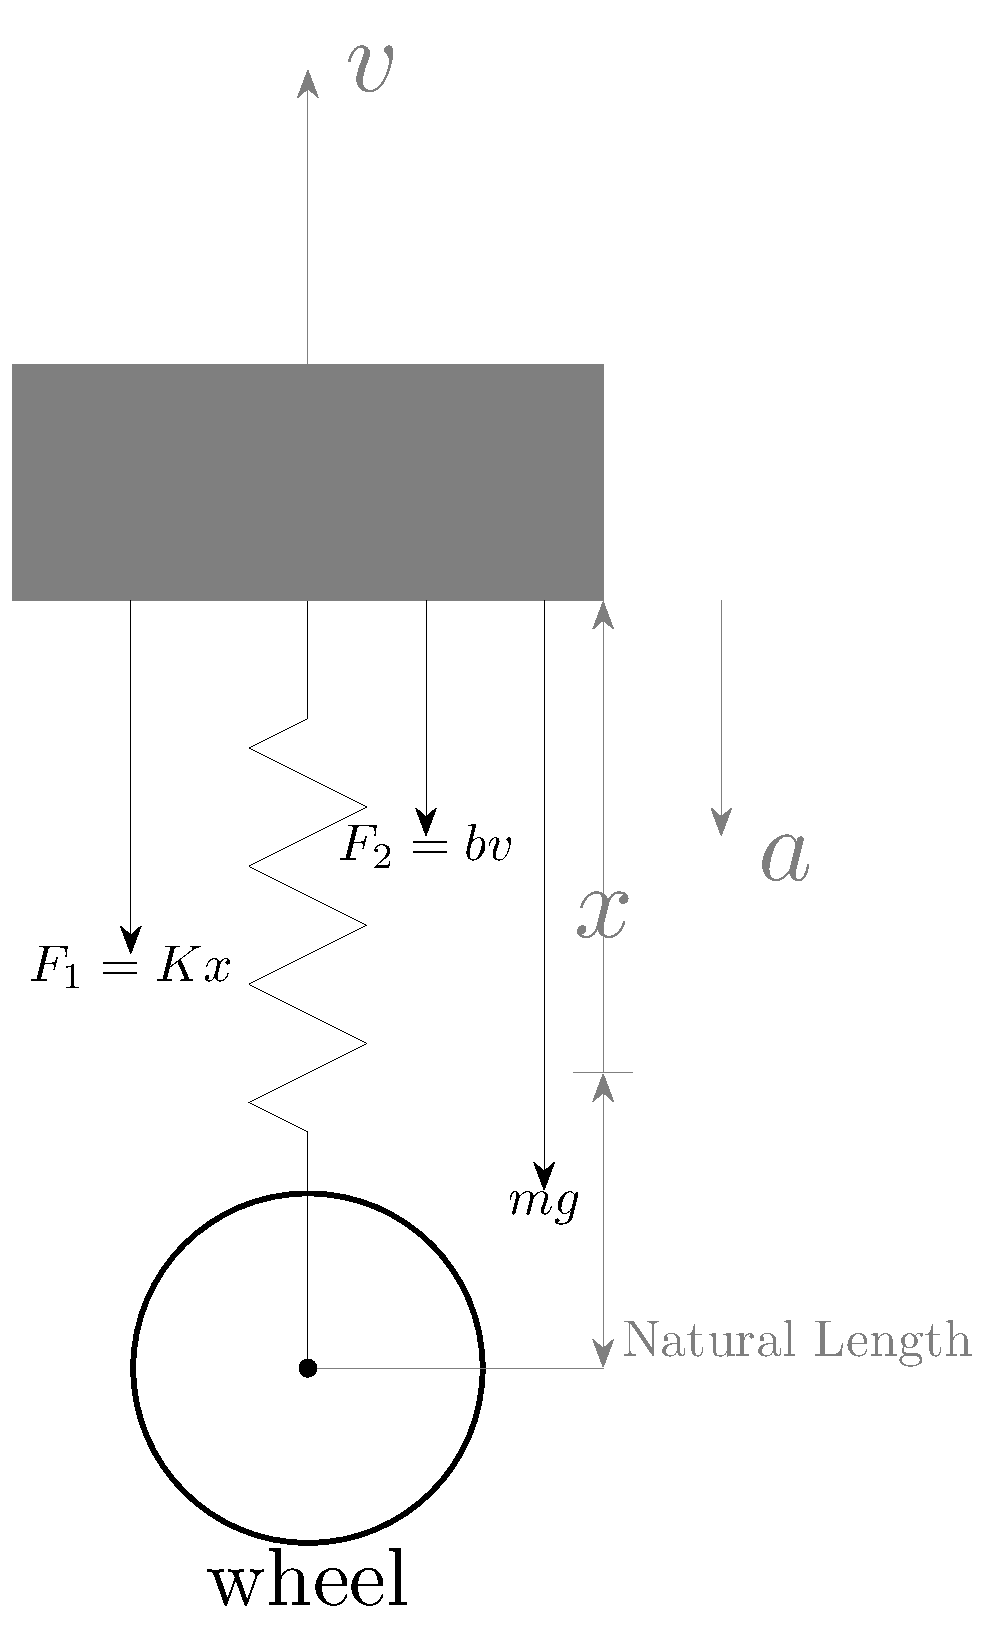
\includegraphics[width=0.8\linewidth]{11_14_21_fbd.pdf}
        \caption{FBD of the damped oscillation system}
        \label{Fig-1}
    \end{figure}

Now, as the oscillation begins, from the \figref{Fig-1} we net force on the mass as,
\begin{align}
    &F=F_{1}+F_{2}+mg\cdot u(t) \label{3}\\
    \Rightarrow &-m\frac{d^2x(t)}{dt^2}=kx(t)+b\frac{dx(t)}{dt}+mg\cdot u(t) \label{4}\\
    \Rightarrow &\frac{d^2x(t)}{dt^2}+\left(\frac{b}{m}\right)\frac{dx(t)}{dt}+\left(\frac{k}{m}\right)x(t)=-g\cdot u(t) \label{5}
\end{align}
Now, taking the Laplace transform on both sides,
\begin{align}
&s^2X(s)+\frac{b}{m}sX(s)+\frac{k}{m}X(s)=-\frac{g}{s} \label{6}\\
\Rightarrow &X(s)=-\frac{g}{s\left(s^2+\frac{b}{m}s+\frac{k}{m}\right)} \label{7}\\
\Rightarrow &X(s)=-\frac{g}{s(s-s_1)(s-s_2)} \label{8}
\end{align}
Where
\begin{align}
&s_1=-\frac{b}{2m}+\sqrt{\left(\frac{b}{2m}\right)^2-\frac{k}{m}} \label{9}\\
&s_2=-\frac{b}{2m}-\sqrt{\left(\frac{b}{2m}\right)^2-\frac{k}{m}} \label{10}
\end{align}
From (8) we get,
\begin{align}
\begin{split}
\Rightarrow &X(s)=\frac{g}{(s_1-s_2)}\left[\frac{1}{s_2(s-s_2)}-\frac{1}{s_1(s-s_1)}\right] \label{11}\\
&+\frac{g}{s_1s_2}\left(\frac{1}{s}\right)
\end{split}
\end{align}
Now again taking the inverse Laplace transform we have,
\begin{align}
&x(t)=\frac{g}{s_1s_2}+\frac{g}{(s_1-s_2)}\left[\frac{1}{s_2}e^{s_2t}-\frac{1}{s_1}e^{s_1t}\right] \label{12}\\
\begin{split}
\Rightarrow &x(t)=\sqrt{\left(\frac{mg}{k}\right)^2+\left(\frac{gb}{2mk}\right)^2}e^{-bt/2m} \\
&\cdot\sin{\left(\sqrt{\frac{k}{m}-\left(\frac{b}{2m}\right)^2}t+\tan^{-1}\left(\frac{2mg\sqrt{\frac{k}{m}-\left(\frac{b}{2m}\right)^2}}{gb}\right)\right)} \\
&+\frac{mg}{k} \label{13}
\end{split}
\end{align}
(Substituting the values of $s_1$ and $s_2$ from \eqref{9} and \eqref{10}) \\
\begin{figure}[h]
    \centering
    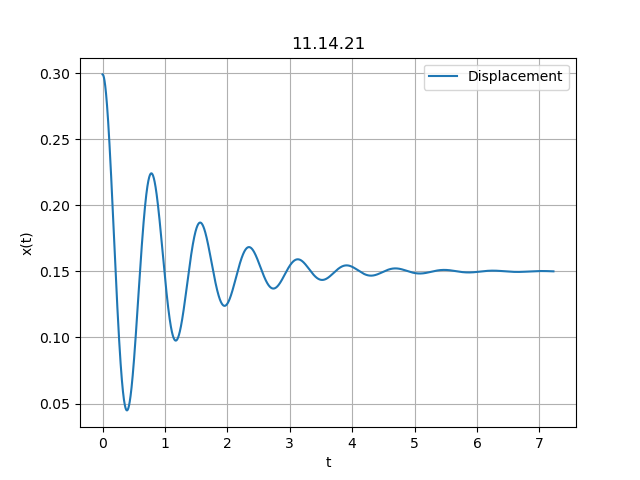
\includegraphics[width=01\linewidth]{11.14.21_plot.png}
    \caption{Displacement  Vs. Time Graph}
    \label{Fig-2}
\end{figure}
From \eqref{13} we have the amplitude after one time period $T$,
\begin{align}
\begin{split}
&\frac{1}{2}\sqrt{\left(\frac{mg}{k}\right)^2+\left(\frac{gb}{2mk}\right)^2}= \\
&\sqrt{\left(\frac{mg}{k}\right)^2+\left(\frac{gb}{2mk}\right)^2}e^{-bT/2m} \label{14}\\
\end{split}
\end{align}
\begin{align}
\Rightarrow &e^{\pi b/\sqrt{mk}}=2 \label{15}\\
\Rightarrow &b=\frac{\sqrt{mk}\ln{2}}{\pi} \label{16}
\end{align}
\textbf{Answer :}
Now substituting the values of the parameters from \tabref{Table-1} we have \\
\begin{enumerate}
\item  The spring constant, $k=4.9\times10^4 \text{N/m}$.
\item  The damping constant, $b=1337.53 \text{Kg/s}$.
\end{enumerate} 
\end{enumerate}
\end{document}
